\documentclass[final,5p,times,twocolumn,authoryear]{elsarticle}

\usepackage{amssymb}
\usepackage{lipsum}
\usepackage{amsthm}
\usepackage{amsmath}
\usepackage[utf8]{inputenc}
\usepackage{lineno}
\usepackage{tabularx}

\newcommand{\pd}[2]{\frac{\partial #1}{\partial #2}}
\newcommand{\pdd}[2]{\frac{\partial^2 #1}{\partial #2^2}}

\journal{Graduate School@UGA}

\begin{document}

\begin{frontmatter}

\title{
\begin{minipage}{0.3\textwidth}

\includegraphics[width=0.9\textwidth]{LEGI-logo.png}
\end{minipage}%
\begin{minipage}{0.4\textwidth}
\centering
\textbf{Simulations of stratified turbulence} \\ \textbf{and comparison with oceanic wave turbulence}
\end{minipage}%
\begin{minipage}{0.3\textwidth}
\flushright

\includegraphics[width=0.9\textwidth]{UGA-logo.png}
\end{minipage}
}

\author[first]{Guillermin Remy}

\begin{abstract}
This study investigates stratified turbulence and its interactions with internal waves using high-resolution Direct Numerical Simulations (DNS). Results reveal an energy cascade following the $k^{-5/3}$ power law, and Richardson number distributions consistent with prior studies.
\end{abstract}

\begin{keyword}
%% keywords here, in the form: keyword \sep keyword, up to a maximum of 6 keywords
Numerical Simulation \sep Fluids Dynamic \sep Turbulence

\end{keyword}

\end{frontmatter}

\section{Introduction}
\label{introduction}

In fluid mechanics, turbulence arises when the Reynolds number, $\mathrm{Re} = UL/\nu \gg 1$, where $U$ and $L$ are the characteristic velocity and length scales of the flow, and $\nu$ is the kinematic viscosity. This condition is typically met in scenarios such as high-speed flows (e.g., jet engine exhaust), large-scale flows (e.g., atmospheric or ocean currents), or in fluids with negligible viscosity, like superfluids. Turbulence is characterised by chaotic, irregular motion that significantly affects the transport of momentum, heat, and mass.

In the context of large-scale climate systems, such as the ocean and atmosphere, turbulence is even more complex due to the additional influence of Earth’s rotation and the stratification of the fluid—either by temperature (in the atmosphere) or density (in the ocean). These factors modify the basic dynamics described by the Navier-Stokes equations. Specifically, stratification leads to the formation of internal waves, which in turn interact with turbulence in intricate ways, driving the transport and mixing processes that are fundamental to climate dynamics.

This project focuses on the effects of density stratification in large-scale flows, particularly how it induces internal wave turbulence. Understanding this phenomenon is crucial because internal waves play a key role in energy transfer within oceans and atmospheres, influencing ocean currents and atmospheric circulation patterns. By studying turbulent flows under stratified conditions, we aim to gain insights into the mechanisms governing large-scale climate dynamics and the energy cascades that drive these systems.

In a first part we will focus on the theory about such flows, we will study the wave in stratified and rotating flows but in our simulation we will only cover the stratified case.

In a second part we will describe the issues faced, how they have been resolved. We will also talk about the simulation parameters.

Finally in the last part we will discuss the results obtained for different simulation. 

\section{Theoretical background}
\subsection{Navier-Stokes Equations}

The governing equations for fluid motion in this study are the Navier-Stokes equations, given by:
\begin{subequations}
\begin{align}
\pd{\rho}{t} + \vec{\nabla} \left( \rho \vec{u} \right) &= 0 \\
\rho \left( \pd{\vec{u}}{t} + \left( \vec{u} \cdot \vec{\nabla} \right) \vec{u} \right) &= - \vec{\nabla} p - \rho g \hat{z} + \mu \Delta \vec{u} - 2 \rho \vec{\Omega} \wedge \vec{u}
\end{align}
\label{eq:NS}
\end{subequations}
where $\rho$ is the fluid density, $\vec{u}$ is the velocity field, $p$ is the pressure, $\mu$ is the dynamic viscosity, $\vec{\Omega}$ is the rotation of the frame of reference and $g$ is the acceleration due to gravity. These equations describe the motion of a viscous fluid, accounting for both inertial and gravitational forces.

\subsection{Dimensionless Numbers}

In the study of fluid mechanics, the Froude number $\mathrm{Fr}$ is a key dimensionless quantity that represents the ratio of inertial forces (advection) to gravitational forces.
\begin{equation*}
	\mathrm{Fr}^2 = U^2 / gH
\end{equation*} 
Here, $U$ is the characteristic velocity, $g$ is gravitational acceleration, and $H$ is the characteristic depth or length scale of the flow. The Froude number is useful in understanding the behaviour of stratified fluids, where gravity plays a significant role in the dynamics.

The Richardson number $Ri$ is a key parameter that characterizes the ratio of buoyancy forces to flow shear forces [\cite{cushman-roisin_introduction_2011}]. This dimensionless number is defined as:
\begin{equation}
Ri = \frac{N^2}{\left(d \bar{u} / dz \right)^2}
\end{equation}

Where $N^2 = -\frac{g}{\rho} \pd{\rho}{z}$ is the Brunt-Väisälä frequency [\cite{pedlosky_geophysical_1979}] and $d \bar{u} / dz$ is the vertical velocity gradient.

For rotating flow we can also define the Rossby number as the ratio of the inertial forces and the Coriolis forces
\begin{equation*}
	Ro = \frac{U}{fL}
\end{equation*}
Here, $f$ is the Coriolis parameter $f = 2\Omega$ in the case of a planar frame of reference, if we look at the case of the Earth, we need to take account for the latitude at which the experiment/simulation takes place.

\subsection{Boussinesq Approximation and Inertia-Wave Propagation}

For density stratified fluids, the Boussinesq approximation [\cite{boussinesq_theorie_1897}] is commonly applied, which assumes that density variations are small and only affect the buoyancy force, while the density is constant elsewhere. After applying this approximation to the Navier-Stokes equations and simplifying, we derive the gravity-wave propagation equation:
\begin{equation}
\partial^2_t \vec{u} = \left( N^2 \nabla^2_h \nabla^{-2} \right) \vec{u} \label{eq:Wave Propagation}
\end{equation}
where $\nabla_h$ is the horizontal gradient operator, $\nabla$ is the spatial gradient operator, and $N$ is the Brunt-Väisälä frequency. This equation describes the propagation of internal waves in a stratified fluid.

\subsection{Dispersion Relation of Gravity Waves}

The dispersion relation for inertia-gravity waves is given by:
\begin{equation}
\omega^2 = \frac{f^2 k_z^2 + N^2 k_h^2}{k^2} \label{eq:Dispersion relation}
\end{equation}
where $\omega$ is the frequency of the wave, $k_z$ is the vertical wave-vector and $k_h^2 = k_x^2 + k_y^2$ is the horizontal wave-vector. This relation shows that the frequency $\omega_+$ is bounded within the range $\left[ f, N \right]$ and $\omega_-$ between $\left[ N, -f \right]$, where $N$ is the Brunt-Väisälä frequency, which determines the stability of stratified fluid systems and $f$ is the Coriolis frequency, which quantifies the rotation of the frame of reference.

\section{Numerical Setup}

\subsection{Computational Tools}

This study leverages \texttt{Fluidsim} [\cite{fluiddyn}], a high-performance computing (HPC) code utilizing pseudo-spectral solvers. \texttt{Fluidsim} is particularly well-suited for simulating fluid dynamics in stratified flows, offering efficient computation for large-scale simulations.

\subsection{Computational Environment}

The simulations are performed on three platforms: 

\begin{itemize}
    \item \textbf{Zen (Mesonet)}: A supercomputer offering ease of use and good computational power for medium-resolution simulations (up to $(256, 256, 64)$). However, it lacks efficient parallelization capabilities for multi-node simulations.
    \item \textbf{GRICAD Cluster (Miniforge3)}: Supports single-node simulations. This will be the primary focus due to the current issues with multi-node setups.
    \item \textbf{GRICAD Cluster (Guix)}: Provides potential for multi-node simulations, which is essential for higher-resolution simulations, but setup and execution currently face technical challenges.
\end{itemize}

\subsection{Challenges Encountered}

Several technical issues have impacted the simulation workflow:

\begin{itemize}
    \item \textbf{GRICAD (Guix):} Initial difficulties arose during configuration, requiring IT support to resolve. Multi-node simulations using MPI processes are not functioning, limiting the scalability needed for high-resolution simulations.
    \item \textbf{Zen (Mesonet):} While job submission is straightforward, parallel simulations using MPI are not currently working. This restricts computational efficiency, as only sequential simulations are possible at present.
\end{itemize}

Addressing these challenges is essential for performing high-resolution DNS efficiently and should be a priority for future work.

\section{Simulation Parameters}

\subsection{Direct Numerical Simulation (DNS) Requirements}

Direct Numerical Simulations (DNS) require high grid resolutions capable of resolving all turbulent scales down to the Kolmogorov length scale $\eta$. This ensures the accurate representation of flow dynamics across the entire spectrum, from large-scale eddies to fine-scale dissipation. 

\subsection{Reynolds Number and Kolmogorov Length Scale}

The Reynolds number $Re_n$ for a viscosity of order $n$ is expressed as:
\begin{equation*}
    Re_n = \frac{U L^{n-1}}{\nu_n},
\end{equation*}
where $\nu_n$ is the viscosity of order $n$. For $n=2$, $\nu_2$ represents the standard viscosity term from the Navier-Stokes equations. Higher-order viscosities ($n>2$) appear as additional dissipation terms of the form $\nu_n \nabla^n$, offering flexibility in controlling dissipation at smaller scales.

Using the turbulent scaling $u(l) = (\varepsilon l)^{1/3}$, the Reynolds number at a given length scale $l$ becomes:
\begin{equation*}
    Re_n(l) = \frac{\varepsilon^{1/3} l^{n - 2/3}}{\nu_n}.
\end{equation*}

The Kolmogorov length scale $\eta_n$, where $Re_n(l) = 1$, is given by:
\begin{equation*}
    \eta_n = \left(\frac{\nu_n}{\varepsilon^{1/3}}\right)^{1 / (n - 2/3)}.
\end{equation*}

\subsection{DNS Feasibility}

For DNS, the condition $k_{\text{max}} \eta > 1$ must be satisfied, where $k_{\text{max}}$ is the maximum resolved wavenumber:
\begin{equation*}
    k_{\text{max}} = \frac{2\pi}{L_x} \frac{n_x}{2}.
\end{equation*}

Assuming $\nu_2 = 10^{-6}$ and $\varepsilon = 1$, the Kolmogorov length scale $\eta_2$ is approximately $10^{-4.5}$. This would require a horizontal resolution of $n_x \approx 30198$ grid points, which is computationally prohibitive for this project.

To achieve DNS with feasible grid resolutions, we modify the viscosity. The required viscosity $\nu$ for a grid spacing $\Delta x = L_x / n_x$ is:
\begin{equation*}
    \nu = C \left(\frac{L_x}{n_x}\right)^{4/3} \varepsilon^{1/3},
\end{equation*}
where $C \sim 1$ is a constant. 

The maximum initial Reynolds number $Re_i$ that can be injected with a maximum velocity $u_i$ at a characteristic length $L=1.0$ is:
\begin{equation*}
    Re_i = \frac{u_i n_x^{4/3}}{C^{4/3} \varepsilon^{1/3}}.
\end{equation*}

These adjustments allow us to perform DNS within the computational limits of this project while maintaining the necessary physical fidelity.


\section{Simulation Results}
\subsection{Isotropic Test Case}

To begin, we perform simulations on a grid resolution of $(256 \times 256 \times 64)$ for a setup without stratification. For this, we use the standard 3D solver from \texttt{Fluidsim}, \texttt{fluidsim.solvers.ns3d}, which is designed for isotropic turbulence. This initial test serves to validate the basic behavior of isotropic turbulence.

\begin{figure}[h]
	\centering
	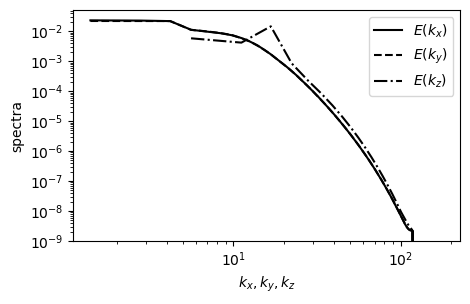
\includegraphics[width=0.41\textwidth]{fig/iso_spectra.png}
	\caption{Energy spectra along each direction for the isotropic case.} 
	\label{fig:iso spectra}
\end{figure}

For both this test and subsequent simulations, we analyze the energy spectra and the energy budget over time. 

Figure \ref{fig:iso spectra} shows the energy transfer from large to small scales. However, due to the relatively low resolution of this simulation, we do not observe a clear inertial range characterized by $E(k) \propto k^{-5/3}$. A higher resolution would likely reveal a more pronounced and extended inertial range.

The energy budget for this test case is displayed in Figure \ref{fig:iso budget}. Here, we observe that the energy distribution is identical across all three directions, confirming the isotropic nature of the turbulence.

\begin{figure}[h]
	\centering
	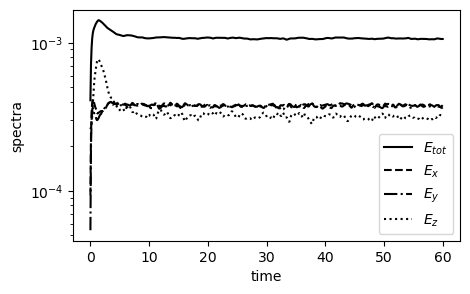
\includegraphics[width=0.5\textwidth]{fig/iso_budget.png}
	\caption{Energy budget along each direction for the isotropic case.} 
	\label{fig:iso budget}
\end{figure}

Summing the contributions from all three directions gives the total energy. The simulation achieves stability after approximately 5 seconds of physical time. This observation allows us to confidently reduce the runtime for subsequent simulations, as the flow reaches a statistically steady state relatively quickly.

\subsection{Stratified Dataset}

We conducted simulations using the solver \texttt{fluidsim.solvers.ns3d.strat}, varying the Brunt-Väisälä frequency $N$ across different cases. The parameters for these simulations are summarized in Table \ref{Table1}.

\begin{table}[h]
\centering
\renewcommand{\arraystretch}{1.5}
\begin{tabularx}{0.48\textwidth}{l c c c c c c } 
 \hline
 Name & Re $\left(\times 10^3\right)$ & Fr & $n_z$ & T & $\tau$ & $k_{\text{max}} \eta$ \\
 \hline \hline
 ns3d-01 & 0.670 & 10 & $64$ & 330 & 60 & 3.14 \\
 ns3d-02 & 0.670 & 5 & $64$ & 225 & 40 & 3.14 \\
 ns3d-05 & 0.670 & 2 & $64$ & 210 & 40 & 3.14 \\
 ns3d-1 & 0.670 & 1 & $64$ & 210 & 40 & 3.14 \\
 ns3d-2 & 0.670 & 0.5 & $64$ & 210 & 40 & 3.14 \\
 ns3d-5 & 0.670 & 0.2 & $64$ & 200 & 60 & 3.14 \\
 ns3d-10 & 0.670 & 0.1 & $64$ & 260 & 60 & 3.14 \\ 
 ns3d-20 & 0.670 & 0.05 & $64$ & 215 & 40 & 3.14 \\ 
 \hline
\end{tabularx}
\caption{Simulation parameters for the stratified dataset. T is the computing time (minutes), $\tau$ is the physical simulation time (seconds).}
\label{Table1}
\end{table}

The Brunt-Väisälä frequency $N$ in each simulation is characterized by its corresponding Froude number, defined as:
\begin{equation*}
    Fr = \frac{\varepsilon^{1/3} l^{4/3}}{N}.
\end{equation*}
The Reynolds number $Re$ is determined by the forcing parameters, with $\varepsilon_{\text{forcing}} = 0.5$ and a forcing wavenumber range of $(k_{\text{min}}, k_{\text{max}}) = (3,4)$. It can be expressed as:
\begin{equation*}
    Re = \frac{2 \pi \varepsilon_{\text{forcing}}}{k_i \nu}.
\end{equation*}
Increasing the grid size would allow higher Reynolds numbers, introducing more complexity to the dataset.

\subsubsection{Dissipation Ratios}

In stratified turbulence, horizontal shears dominate over vertical motions. To examine this, we plot the temporal evolution of the ratio between vertical and horizontal dissipation for each case (Figure \ref{fig:kzkh dissipation}). 
\begin{figure}[h]
	\centering
	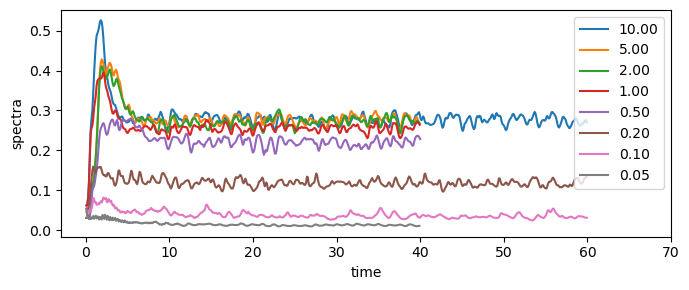
\includegraphics[width=0.5\textwidth]{fig/kzkhdissipation.png}
	\caption{Temporal evolution of the ratio between vertical and horizontal dissipation for each simulation.} 
	\label{fig:kzkh dissipation}
\end{figure}

After an initial buildup phase lasting around 5 seconds, the dissipation ratio stabilizes. The mean dissipation ratio, computed over the stabilized phase, is plotted as a function of the Froude number in Figure \ref{fig:kzkh Froude}.
\begin{figure}[h]
	\centering
	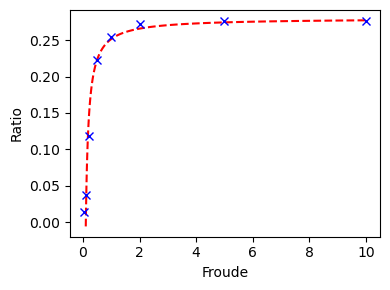
\includegraphics[width=0.4\textwidth]{fig/kzkhFr.png}
	\caption{Mean ratio of vertical to horizontal dissipation as a function of the Froude number. The red dashed line represents the interpolation $y(x) = -1/(35x) + 2.8$.} 
	\label{fig:kzkh Froude}
\end{figure}

The results show a strong dependency on the Froude number. For $Fr < 1$, the dissipation ratio decreases sharply, reaching a ceiling value of approximately $0.28$ for larger $Fr$. This implies that under strong stratification, vertical dissipation becomes negligible compared to horizontal dissipation

\section{Discussion}

This study demonstrates how density stratification modifies turbulence, suppressing vertical motion while enhancing horizontal dynamics. The results confirm that stratification introduces strong anisotropy, reducing vertical dissipation and altering the energy cascade. Intermittent mixing events occur when turbulent forces overcome buoyancy, highlighting the balance between energy input and dissipation under stratified conditions. These findings align with existing theoretical predictions and provide quantitative insights into the behavior of turbulent flows under varying Froude numbers.

However, the study’s scope is constrained by computational limitations, such as restricted Reynolds numbers and simplified boundary conditions. These constraints limit the ability to fully capture the small-scale dynamics and long-term evolution of stratified turbulence. Future work should prioritize higher-resolution simulations, extended parameter ranges, and the inclusion of rotational effects to bridge the gap between idealized models and real-world geophysical systems.

\section{Summary and conclusions}

This work investigates the impact of density stratification on turbulence, showing that stratification induces anisotropy by suppressing vertical motions while driving horizontal energy cascades. The results emphasize the role of the Froude number in governing dissipation ratios and mixing efficiency in stratified flows.

Despite the simplified setup and computational constraints, this study provides a foundation for understanding the dynamics of stratified turbulence and its relevance to geophysical processes. Future efforts should focus on expanding the parameter space and improving computational methods to gain deeper insights into wave-turbulence interactions and their role in large-scale energy transfer and mixing.

\qquad 

\bibliographystyle{elsarticle-harv} 
\bibliography{references.bib}


\end{document}

\endinput